\section{レポート課題3}
\subsection{課題1}
ロジスティク写像の初期変動の影響がないリターンマップを描くためのプログラムを作成し、個体数変動のリターンマップを表示せよ。このとき $r$ は、$r = 1.50, r = 2.60, r = 3.20, r = 3.50, r = 3.86, r = 3.90$ のとし、初期値$x_0$はランダムに与えなさい。グラフは、授業資料を参考として、 $x_{n+1} = r(1 − x_n)x_n、x_{n+1} = x_n$ も同時に描画し、縦軸と横軸は $0~1$ の範囲で出力すること。\\
画像:\\
\begin{figure}[htbp]
  \begin{tabular}{cc}
    \begin{minipage}[t]{0.45\hsize}
      \centering
      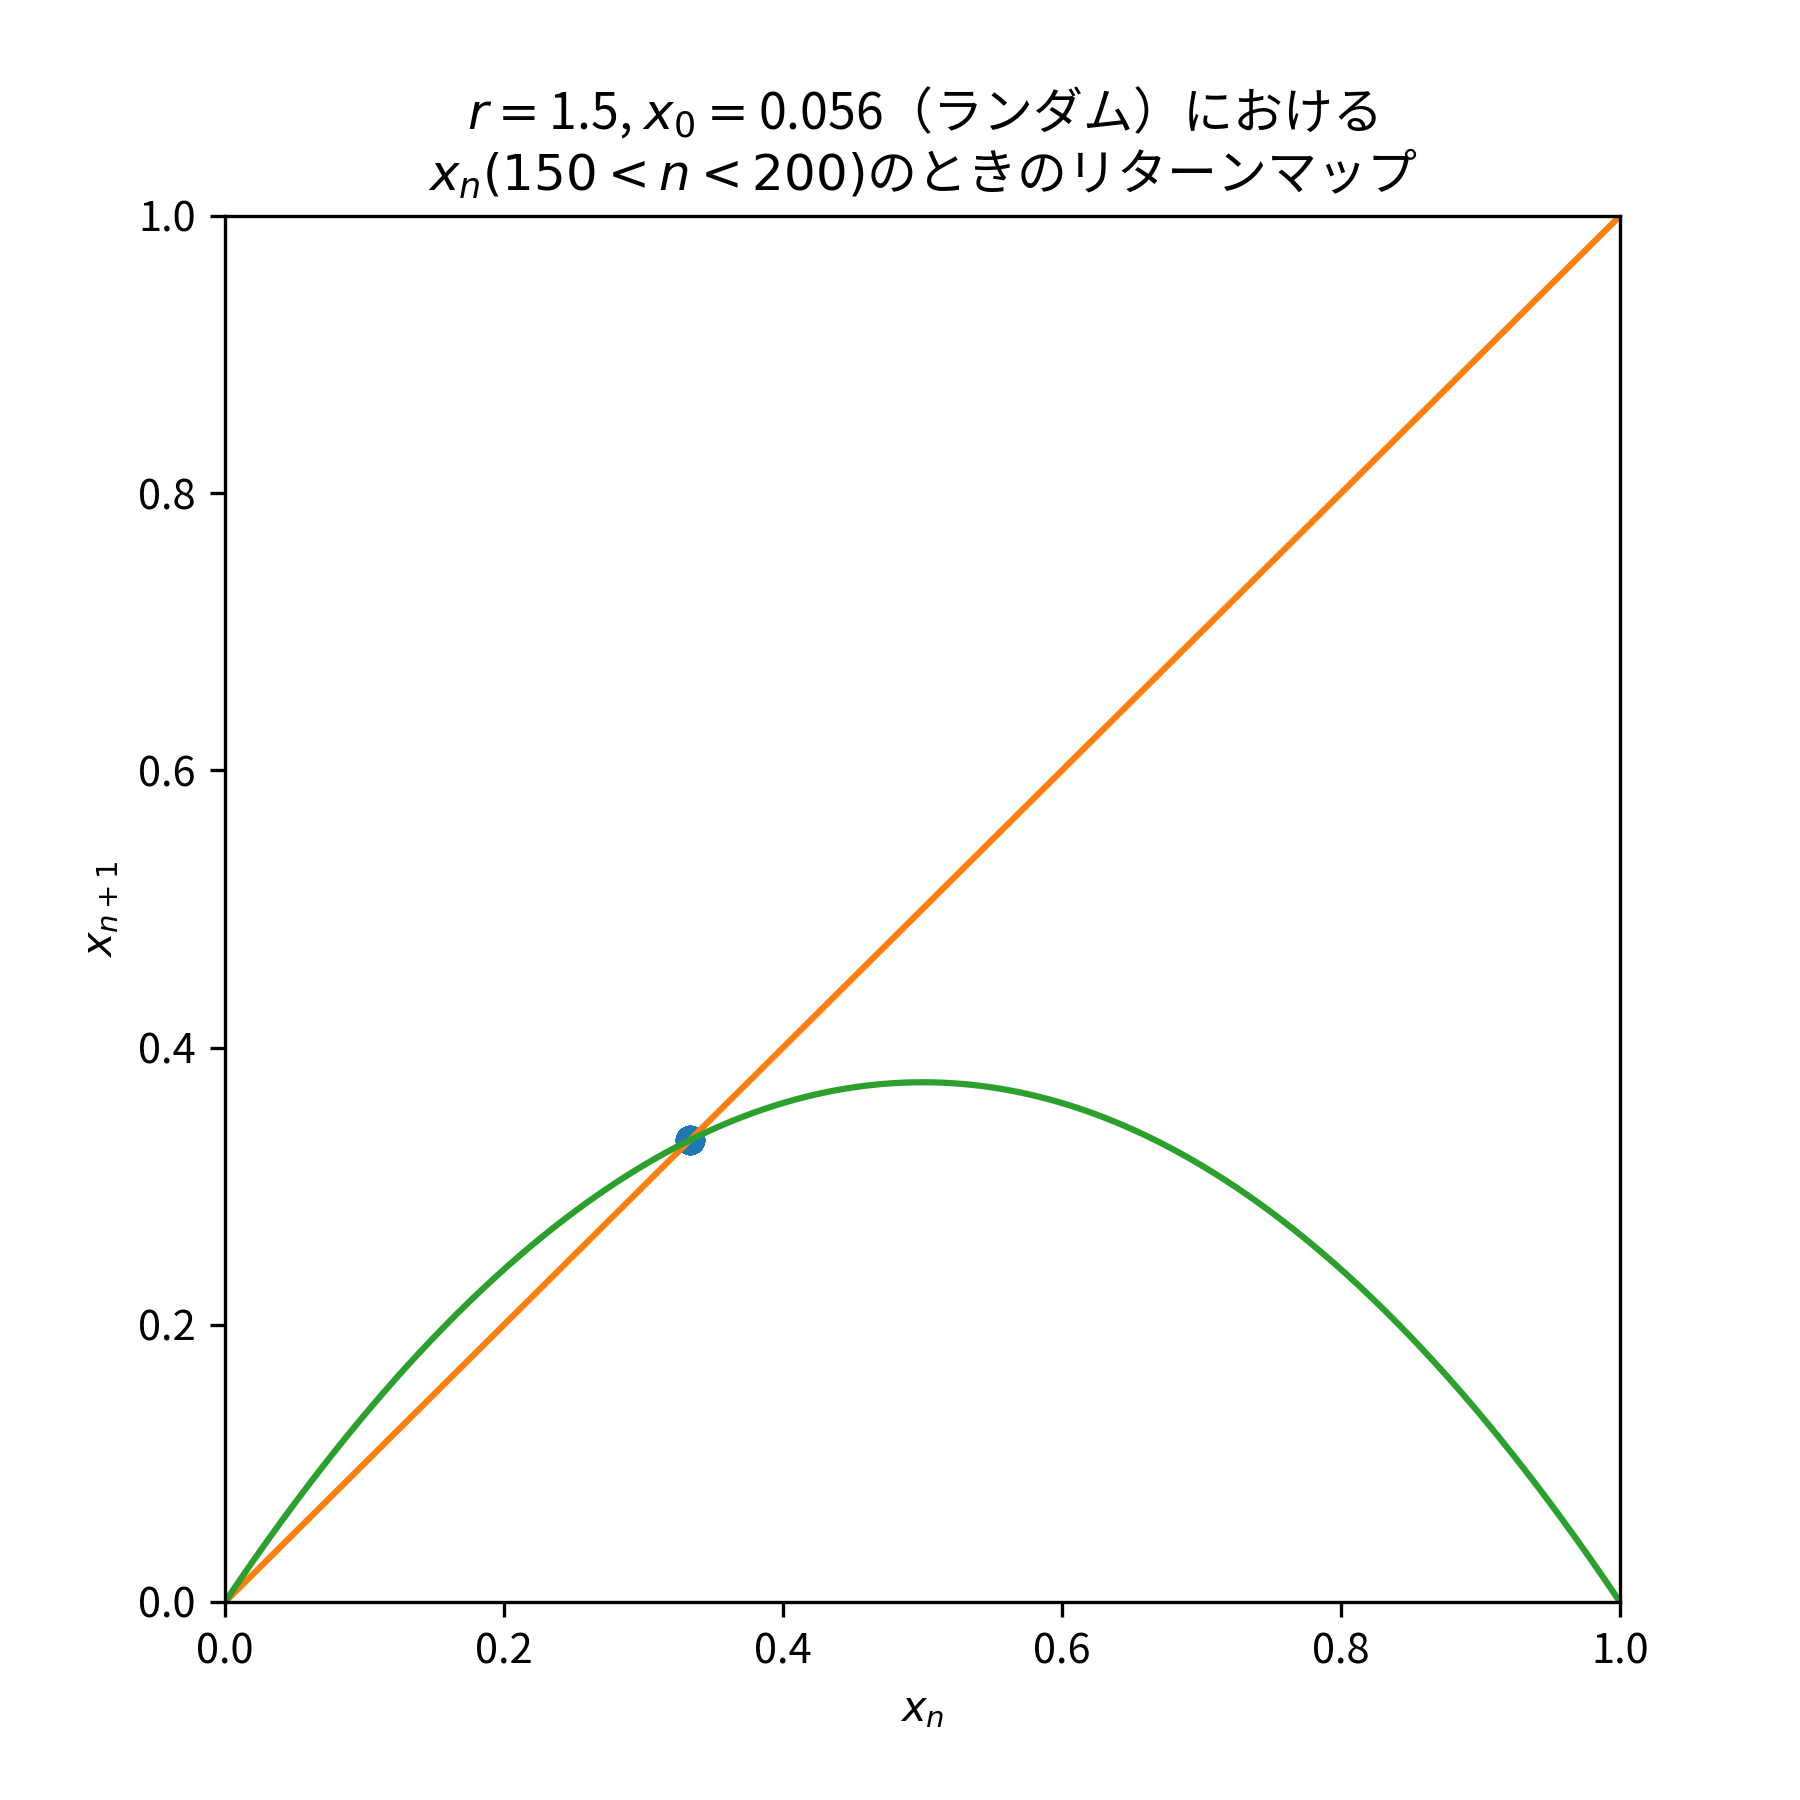
\includegraphics[keepaspectratio, scale=0.3]{images/Problem3/report4_1.png}
    \end{minipage} &
    \begin{minipage}[t]{0.45\hsize}
      \centering
      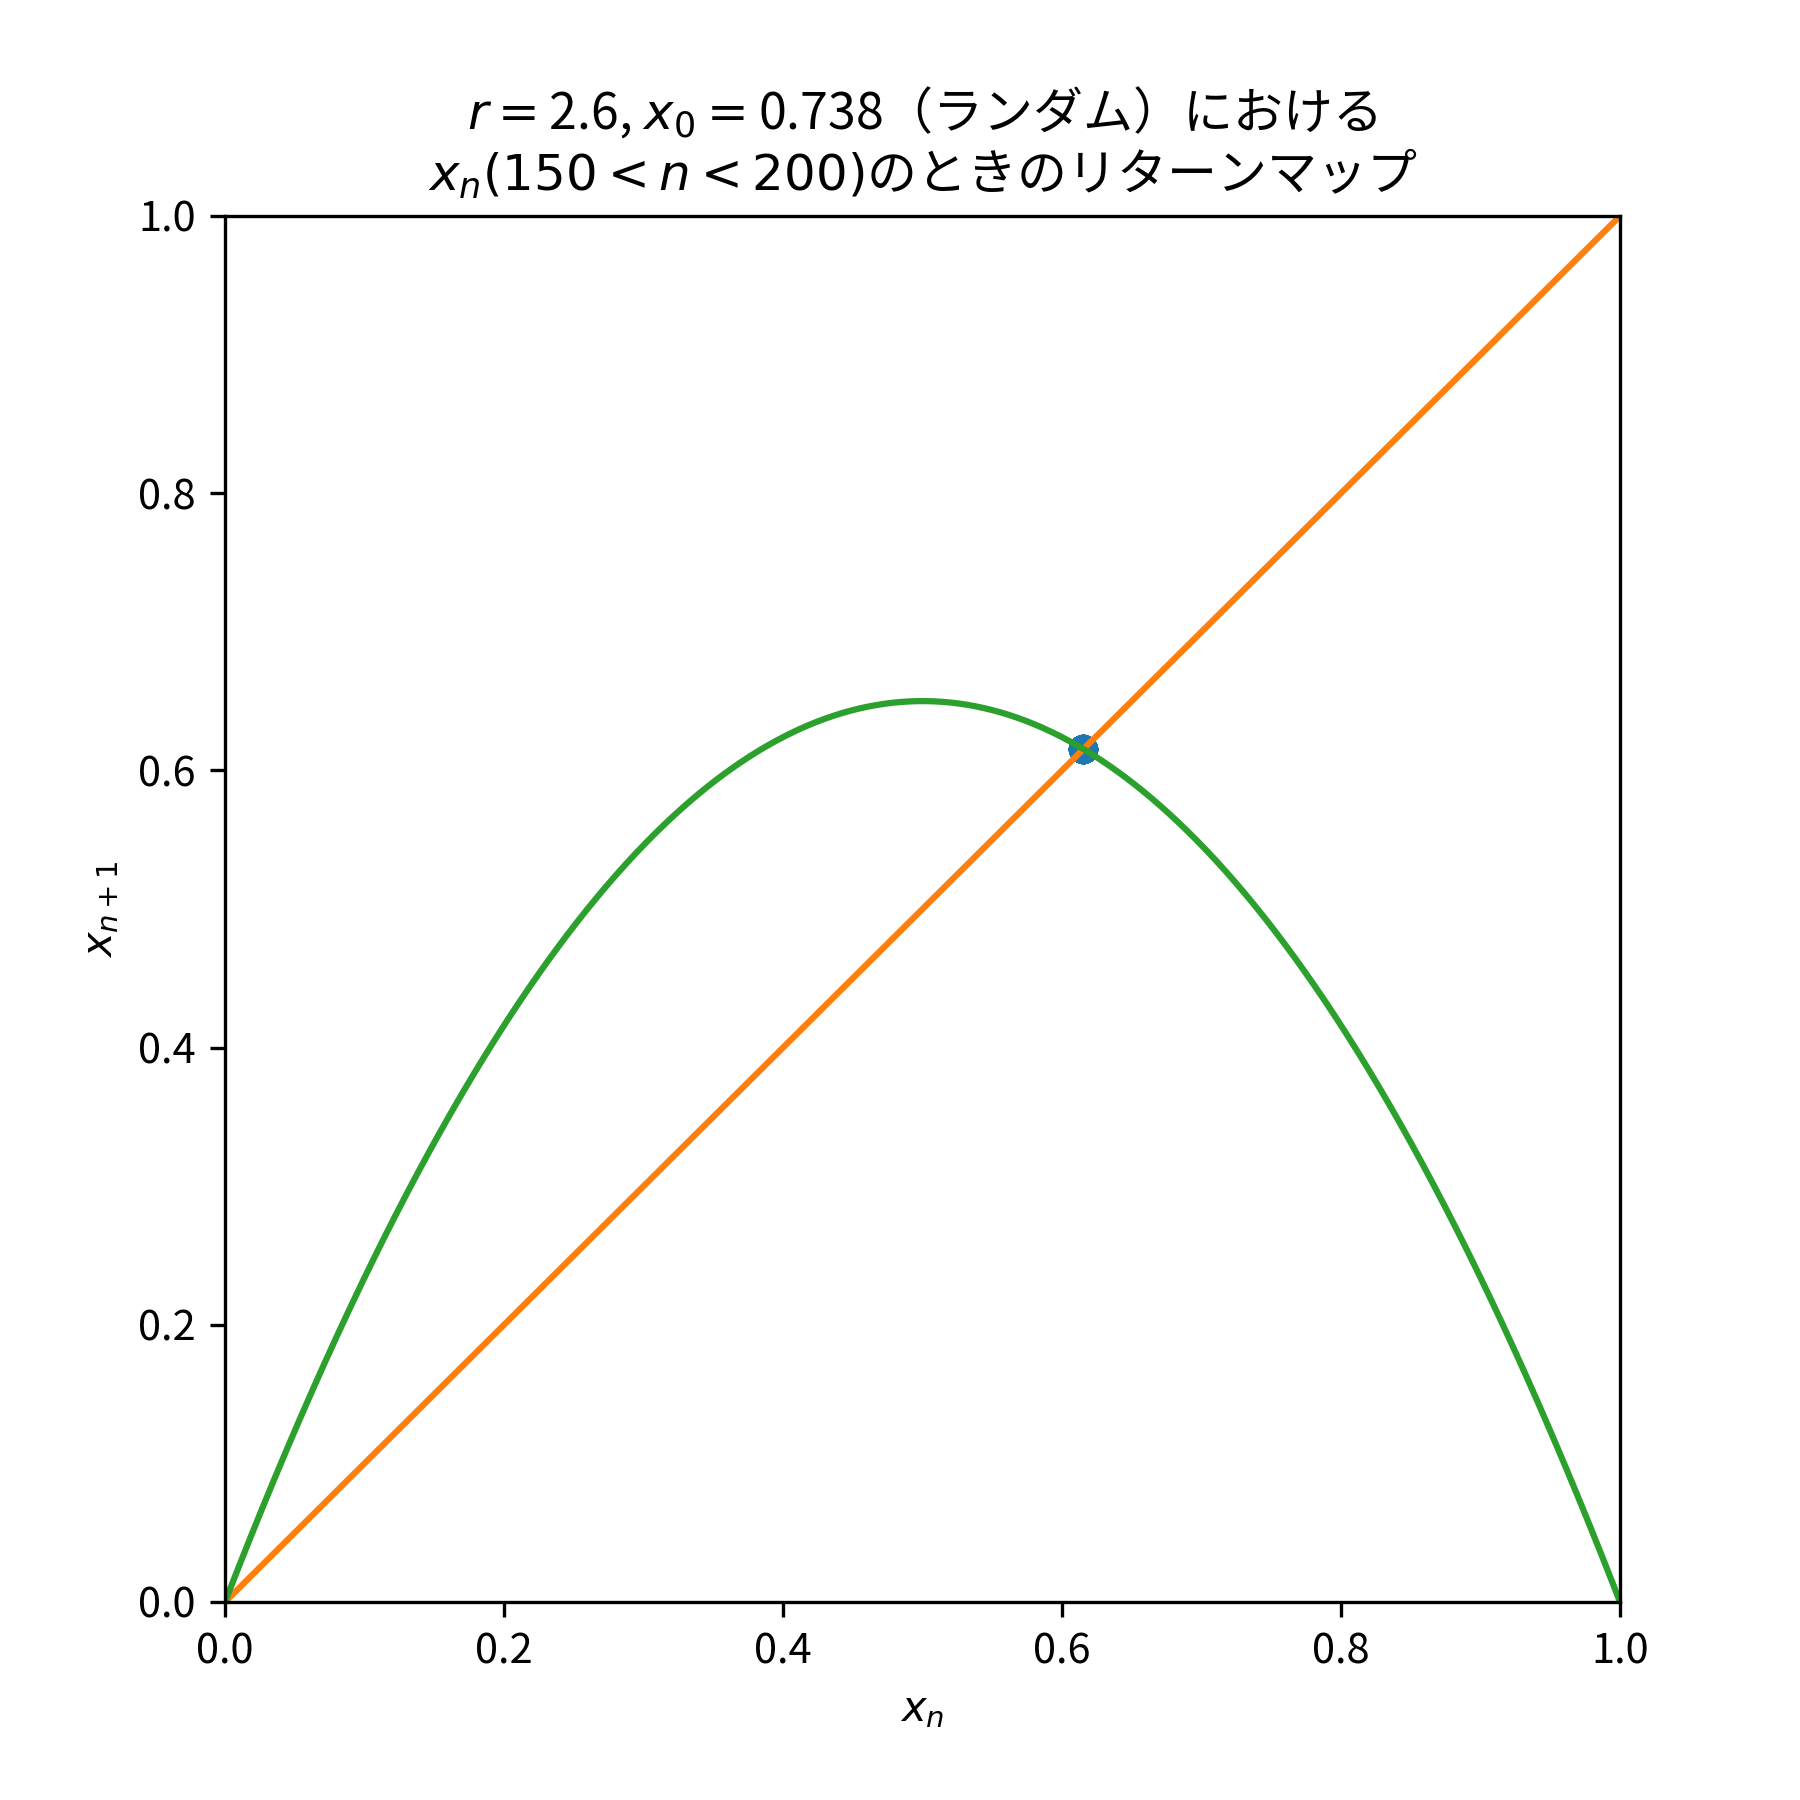
\includegraphics[keepaspectratio, scale=0.3]{images/Problem3/report4_2.png}
    \end{minipage} \\

    \begin{minipage}[t]{0.45\hsize}
      \centering
      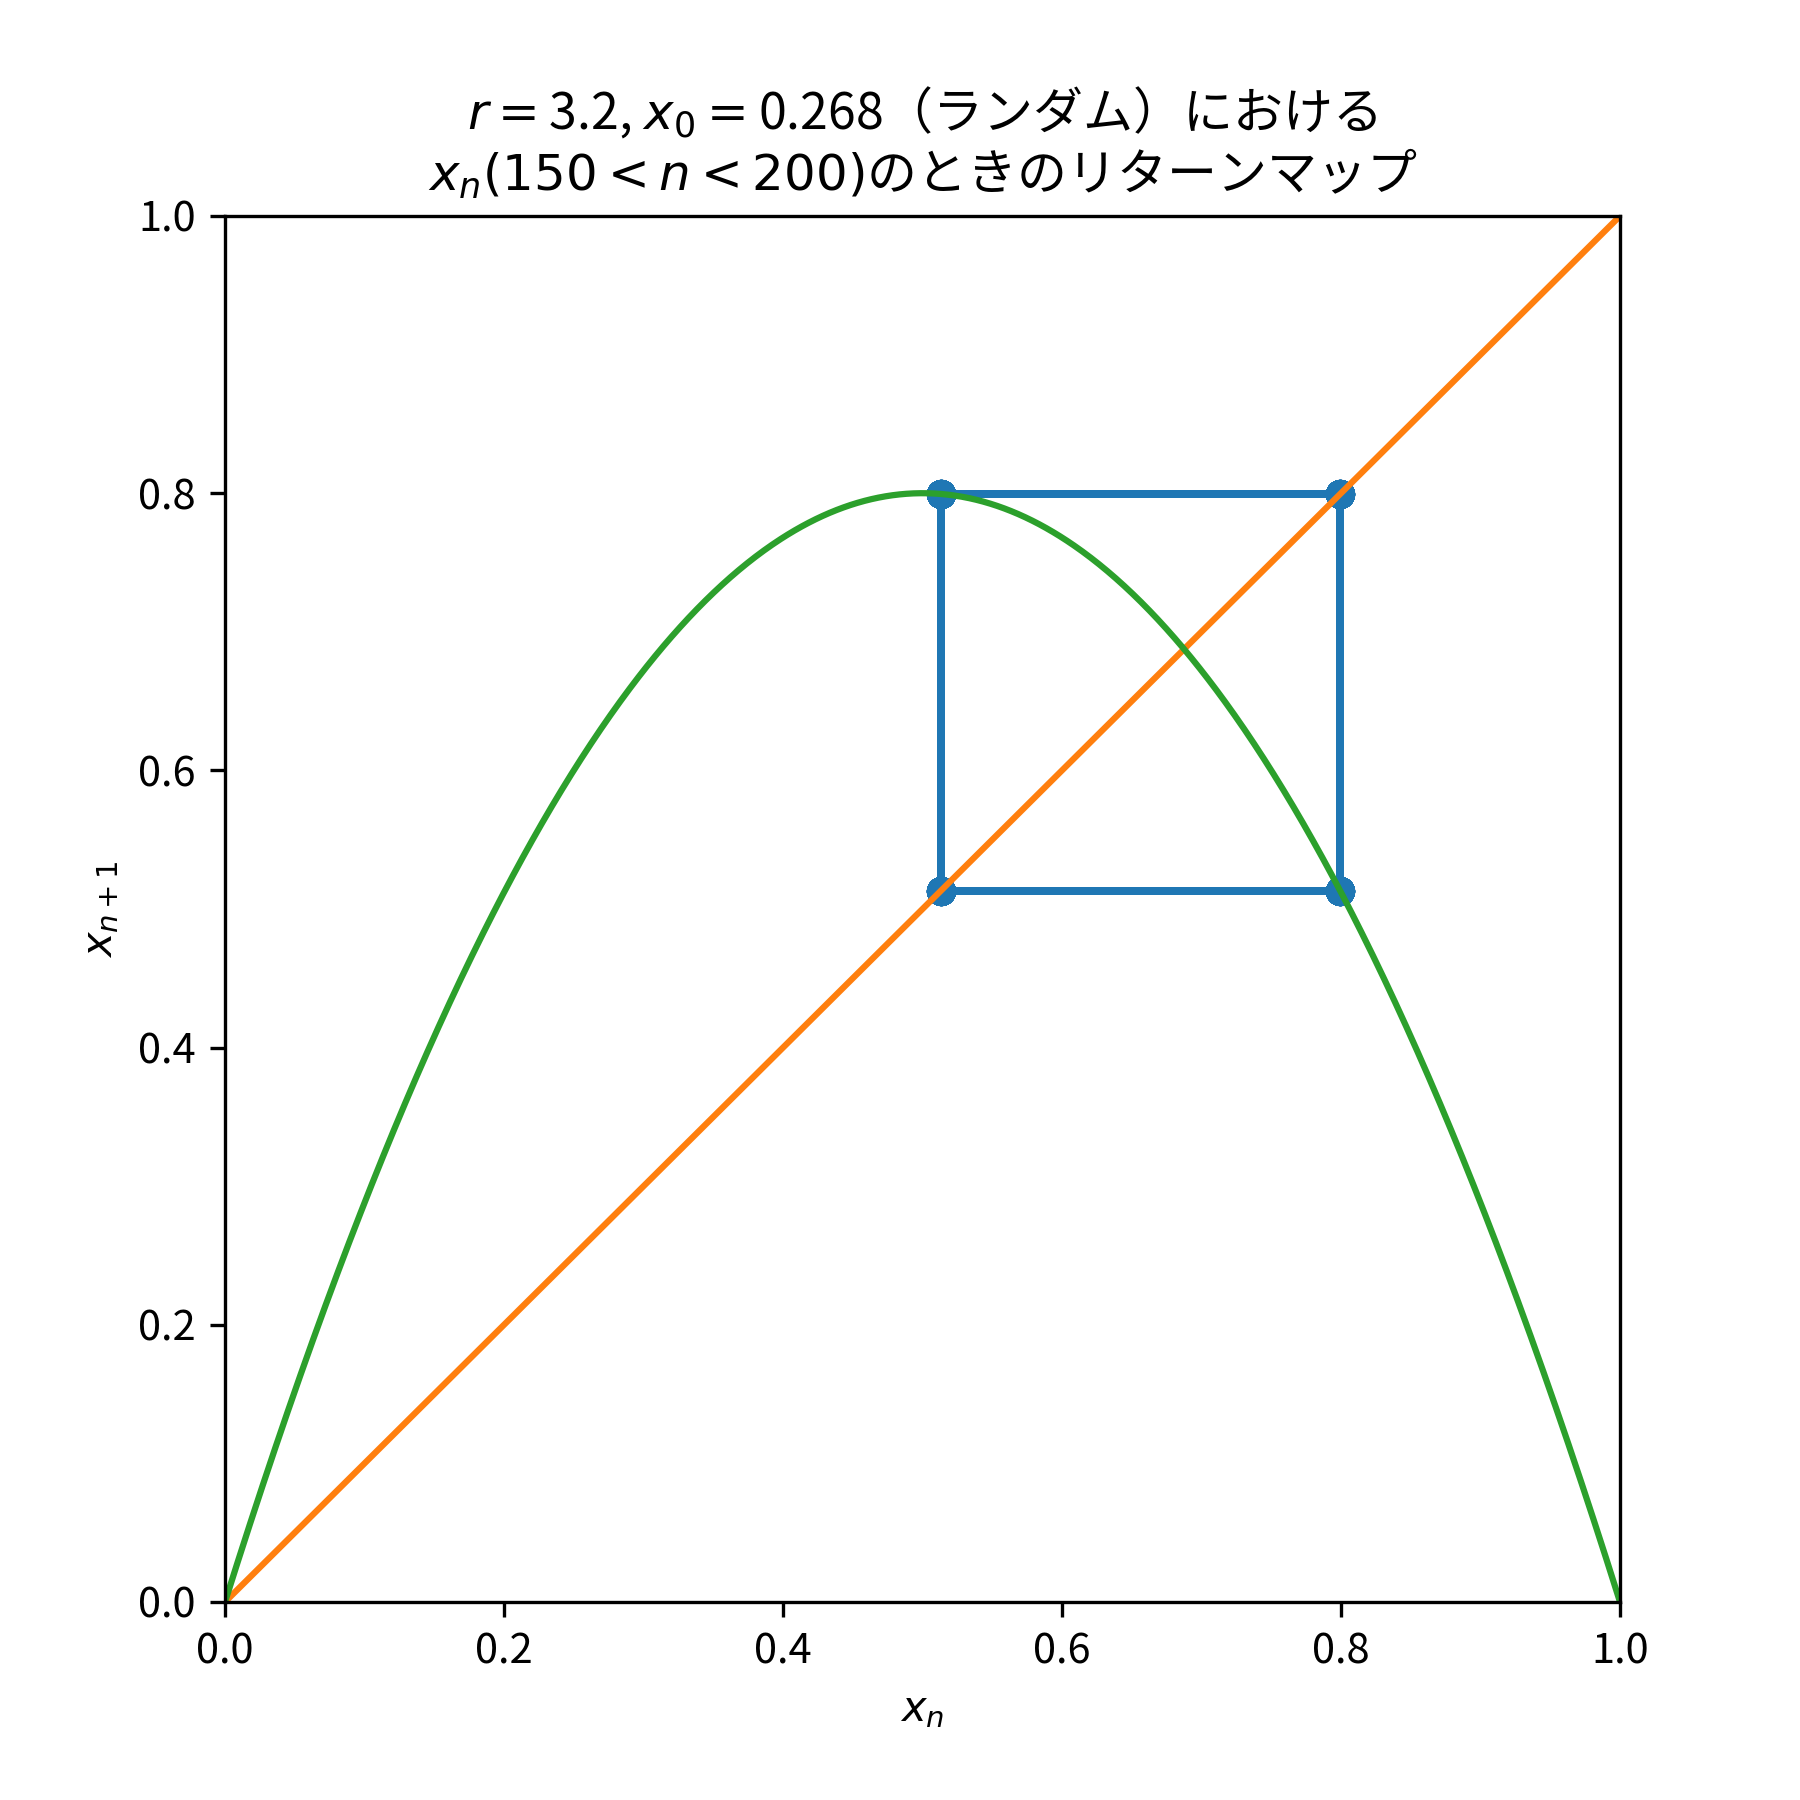
\includegraphics[keepaspectratio, scale=0.3]{images/Problem3/report4_3.png}
    \end{minipage} &
    \begin{minipage}[t]{0.45\hsize}
      \centering
      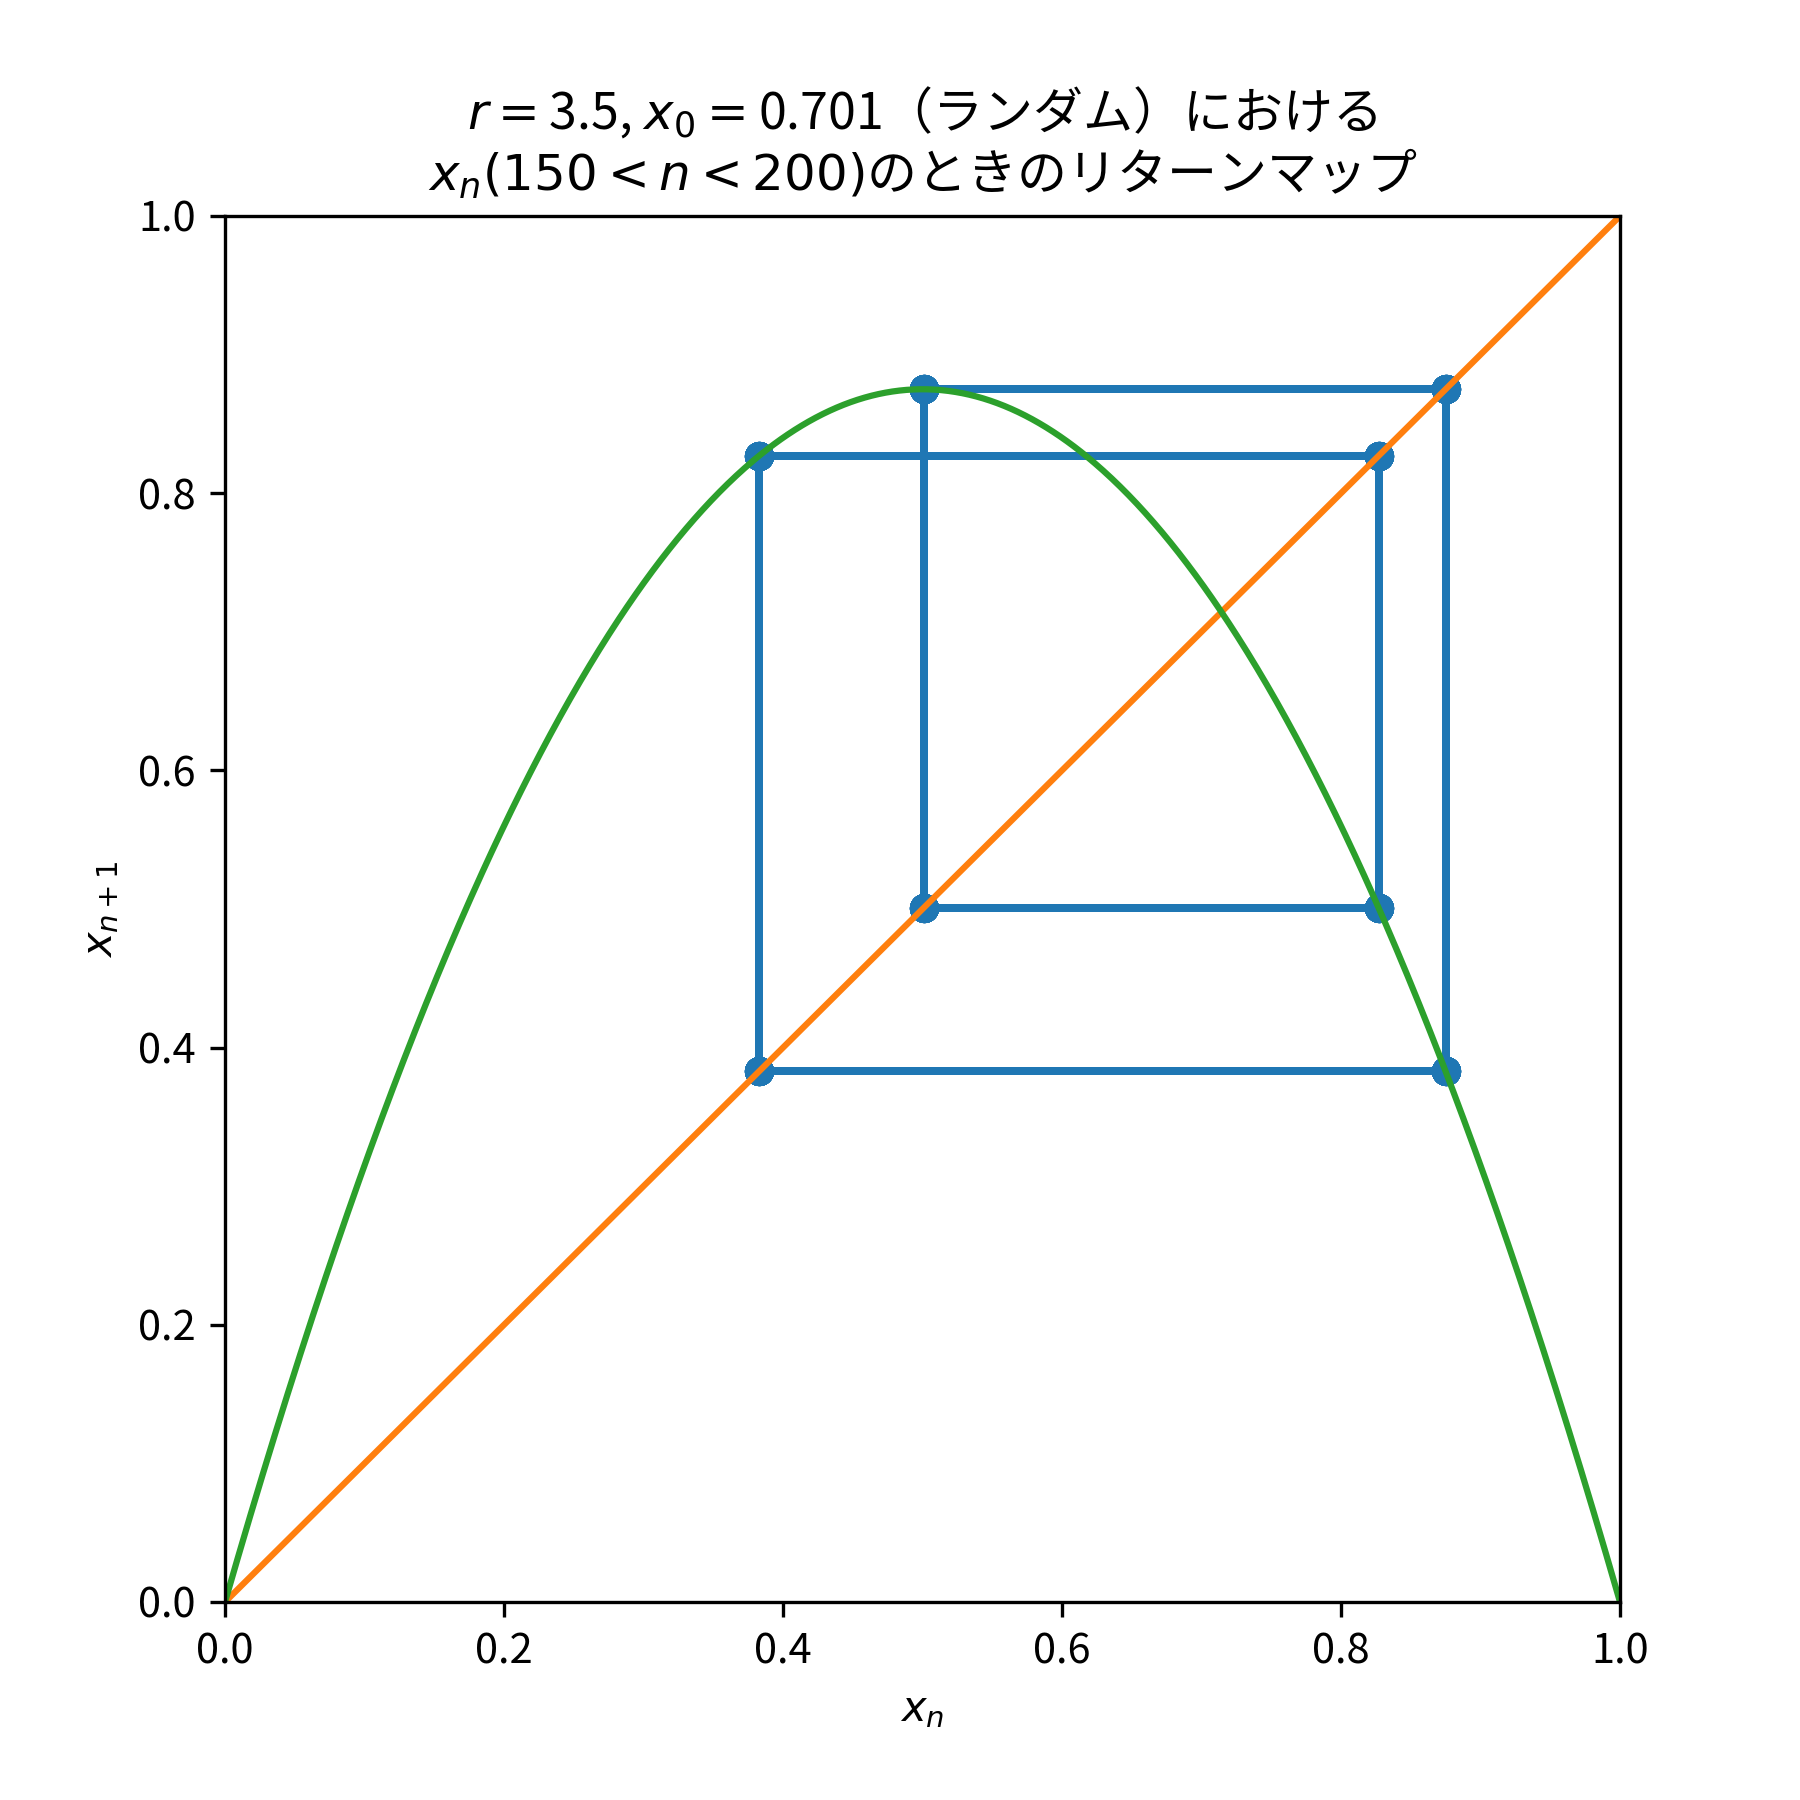
\includegraphics[keepaspectratio, scale=0.3]{images/Problem3/report4_4.png}
    \end{minipage} \\

    \begin{minipage}[t]{0.45\hsize}
      \centering
      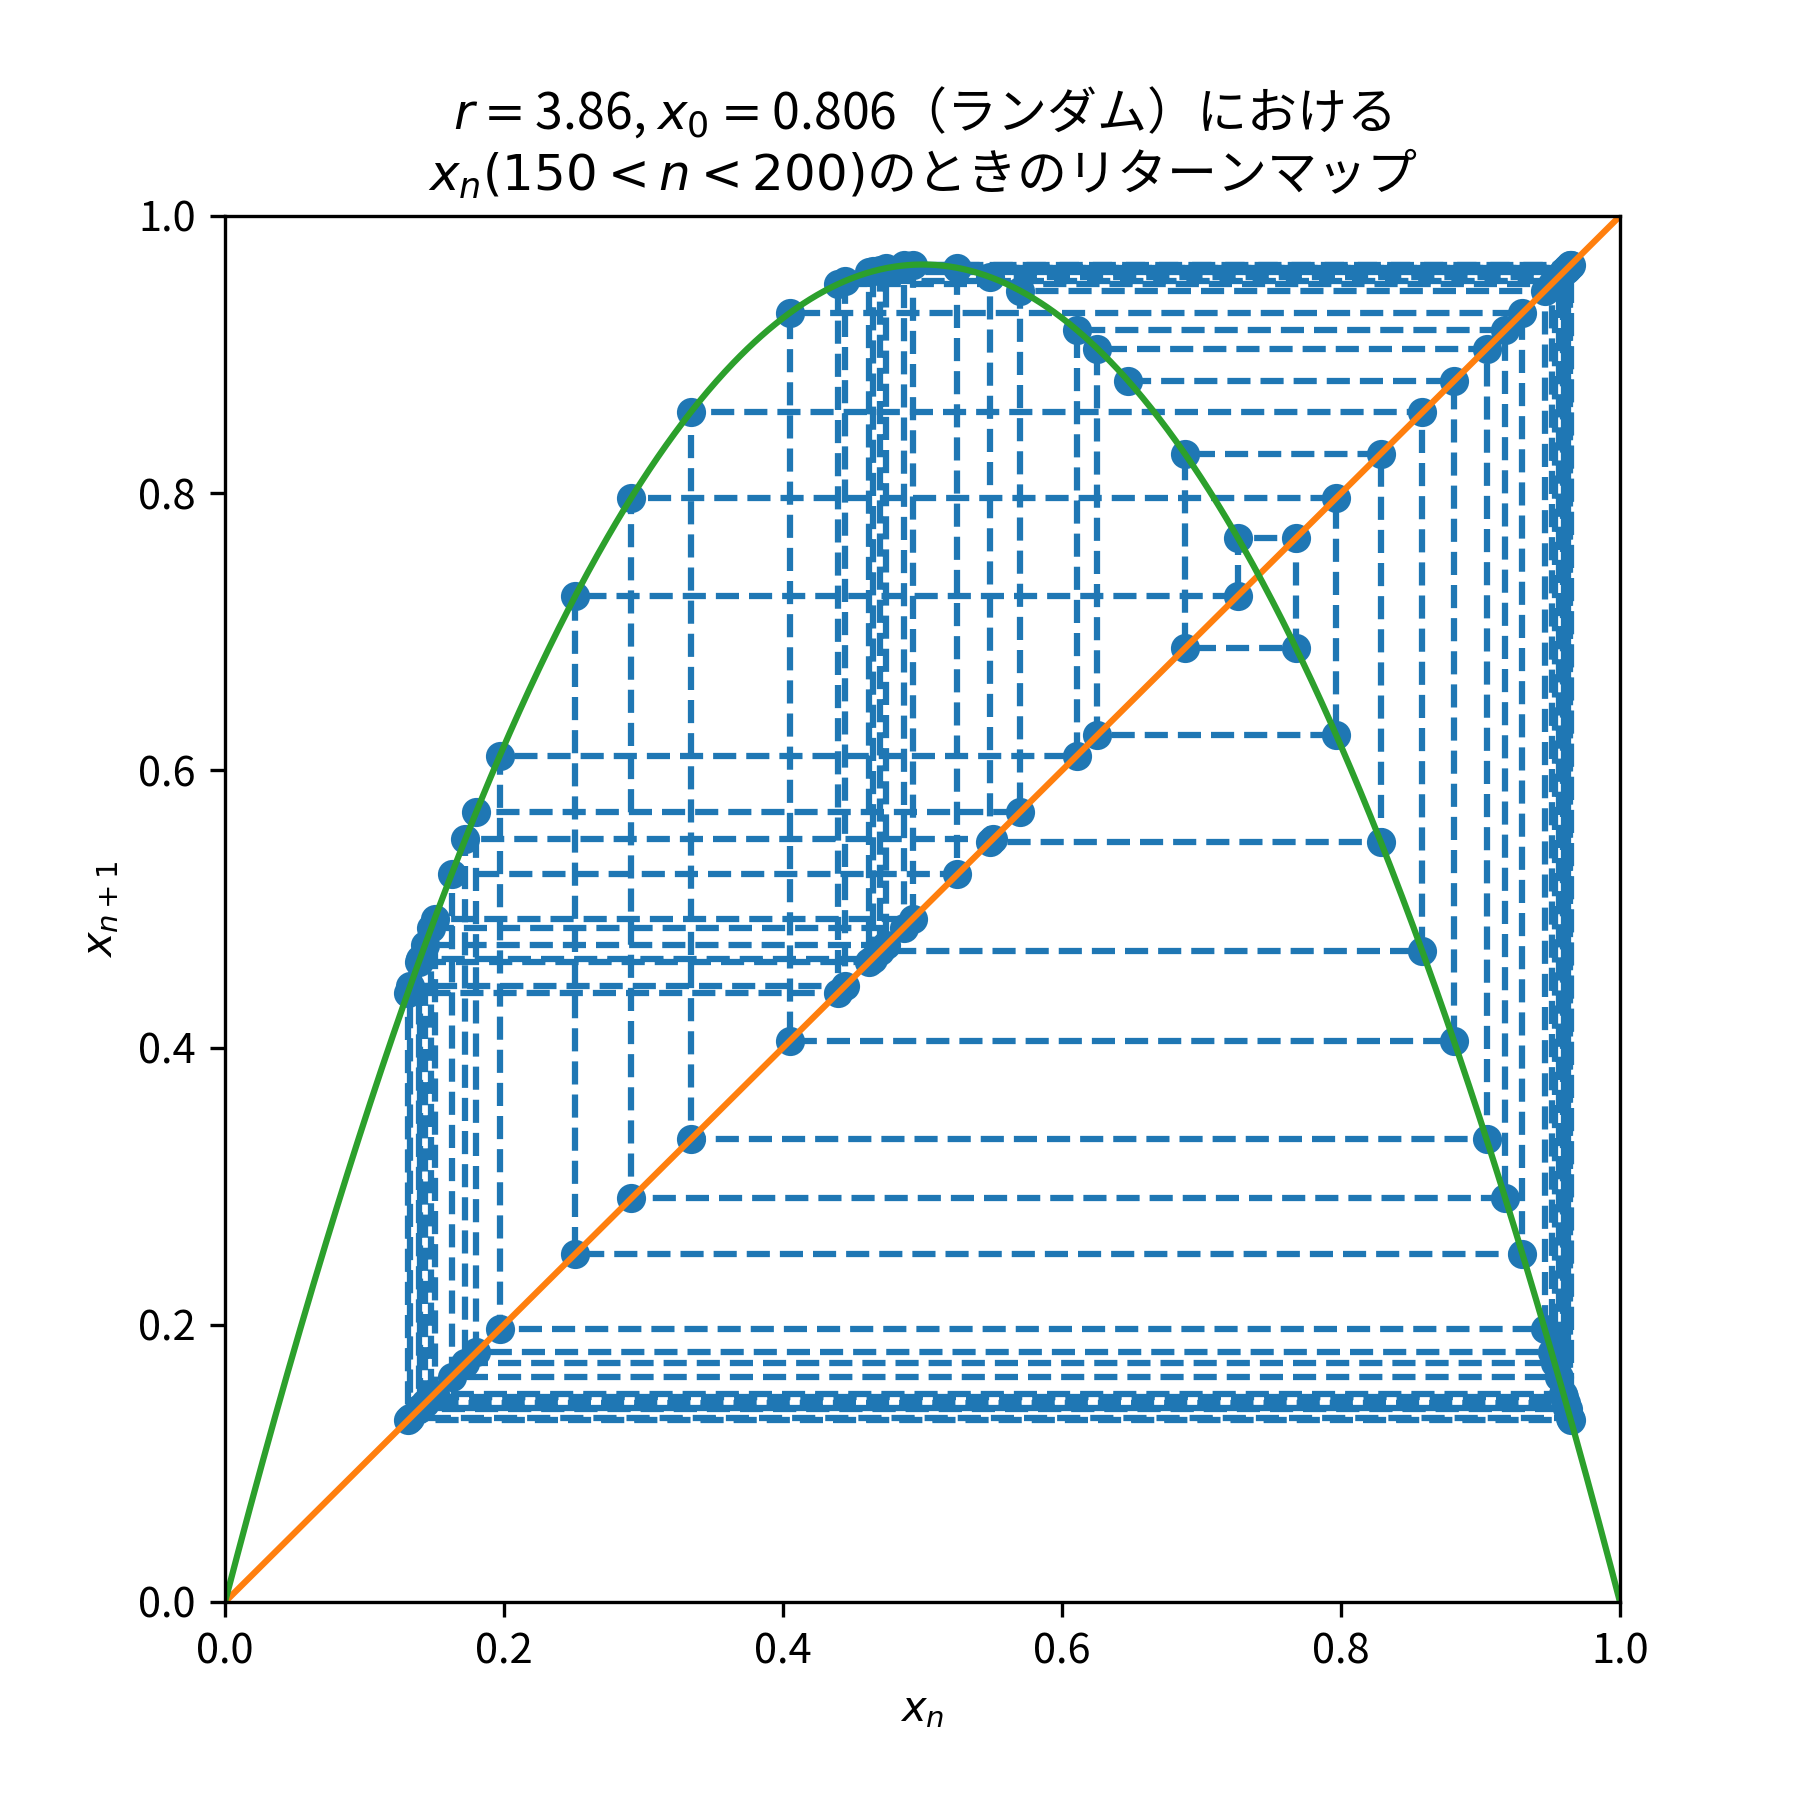
\includegraphics[keepaspectratio, scale=0.3]{images/Problem3/report4_5.png}
    \end{minipage} &
    \begin{minipage}[t]{0.45\hsize}
      \centering
      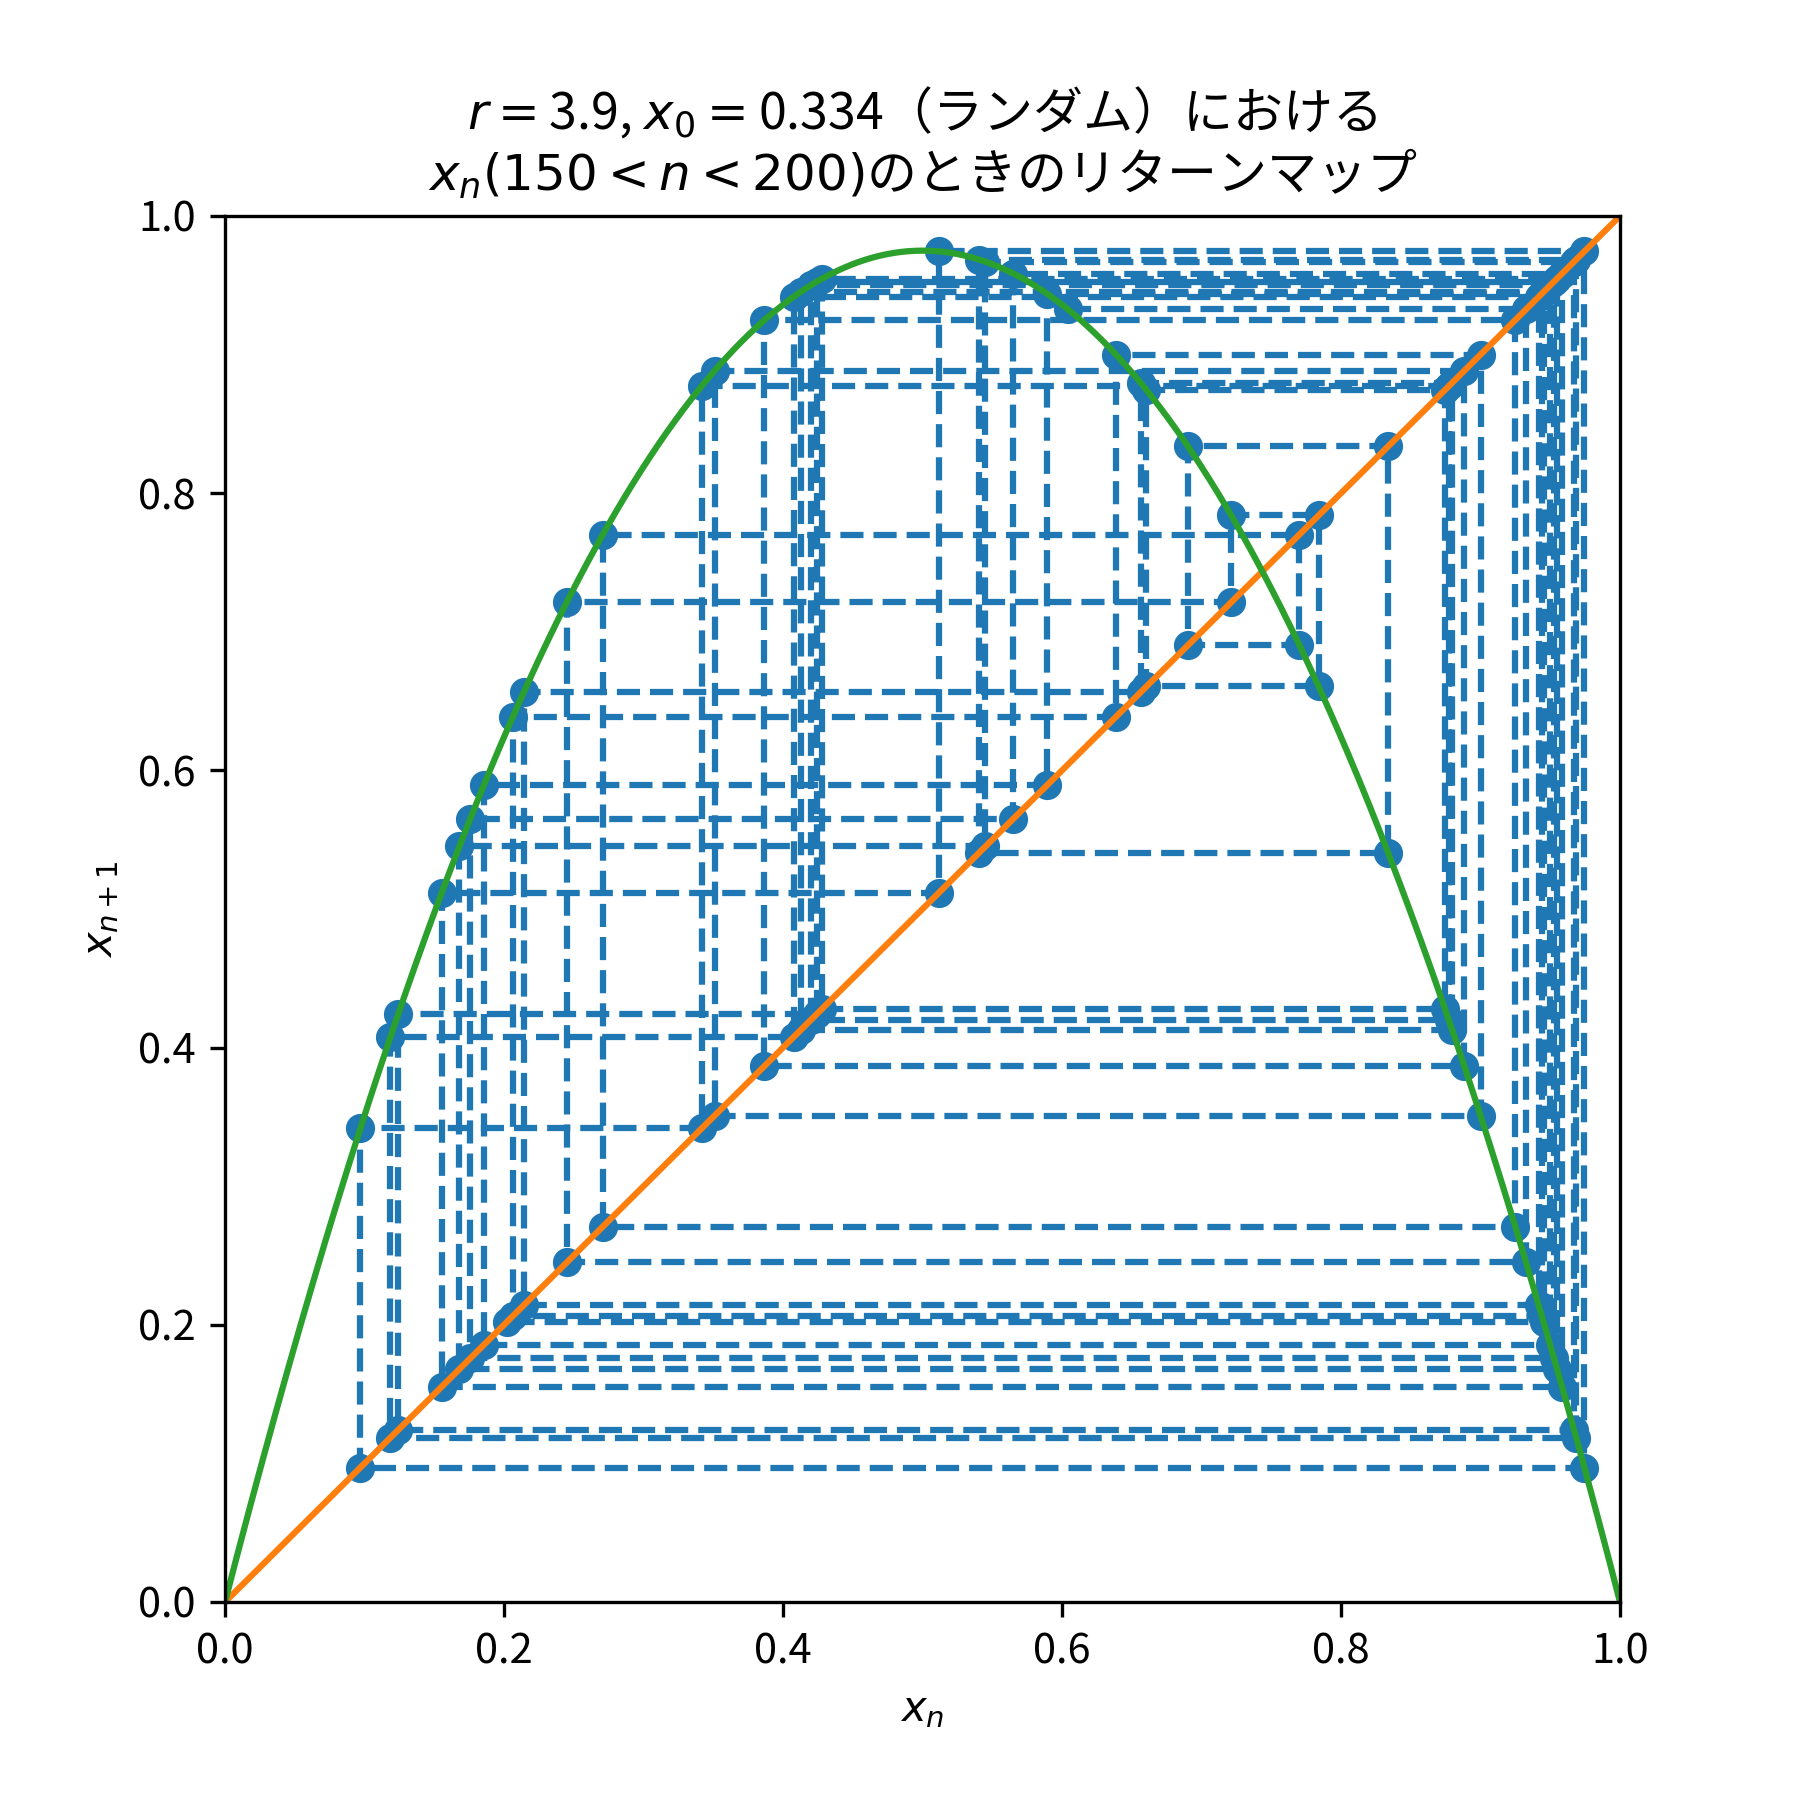
\includegraphics[keepaspectratio, scale=0.3]{images/Problem3/report4_6.png}
    \end{minipage}
  \end{tabular}
\end{figure}
\\
結果:\\
この画像から読み取れた。\\\\
考察:\\
これらの結果から考察することができる。


\subsection{課題2}
$r$ が $1~4$ のときのロジスティク写像の分岐図を描け。また、分岐図の中で3周期の窓が現れている $r$ の範囲を抽出して、グラフを描け。このとき、両グラフとも $r$ は各自適切な刻み幅を設定し、各 $r$ について初期値$x_0$をランダムに与えること。プログラムのソースコードは、 $r$ が $1~4$ のときの分岐図を出力するものと3周期の窓を出力するものとの2つを記載すること。\\
画像:\\
\begin{figure}[htbp]
  \centering
  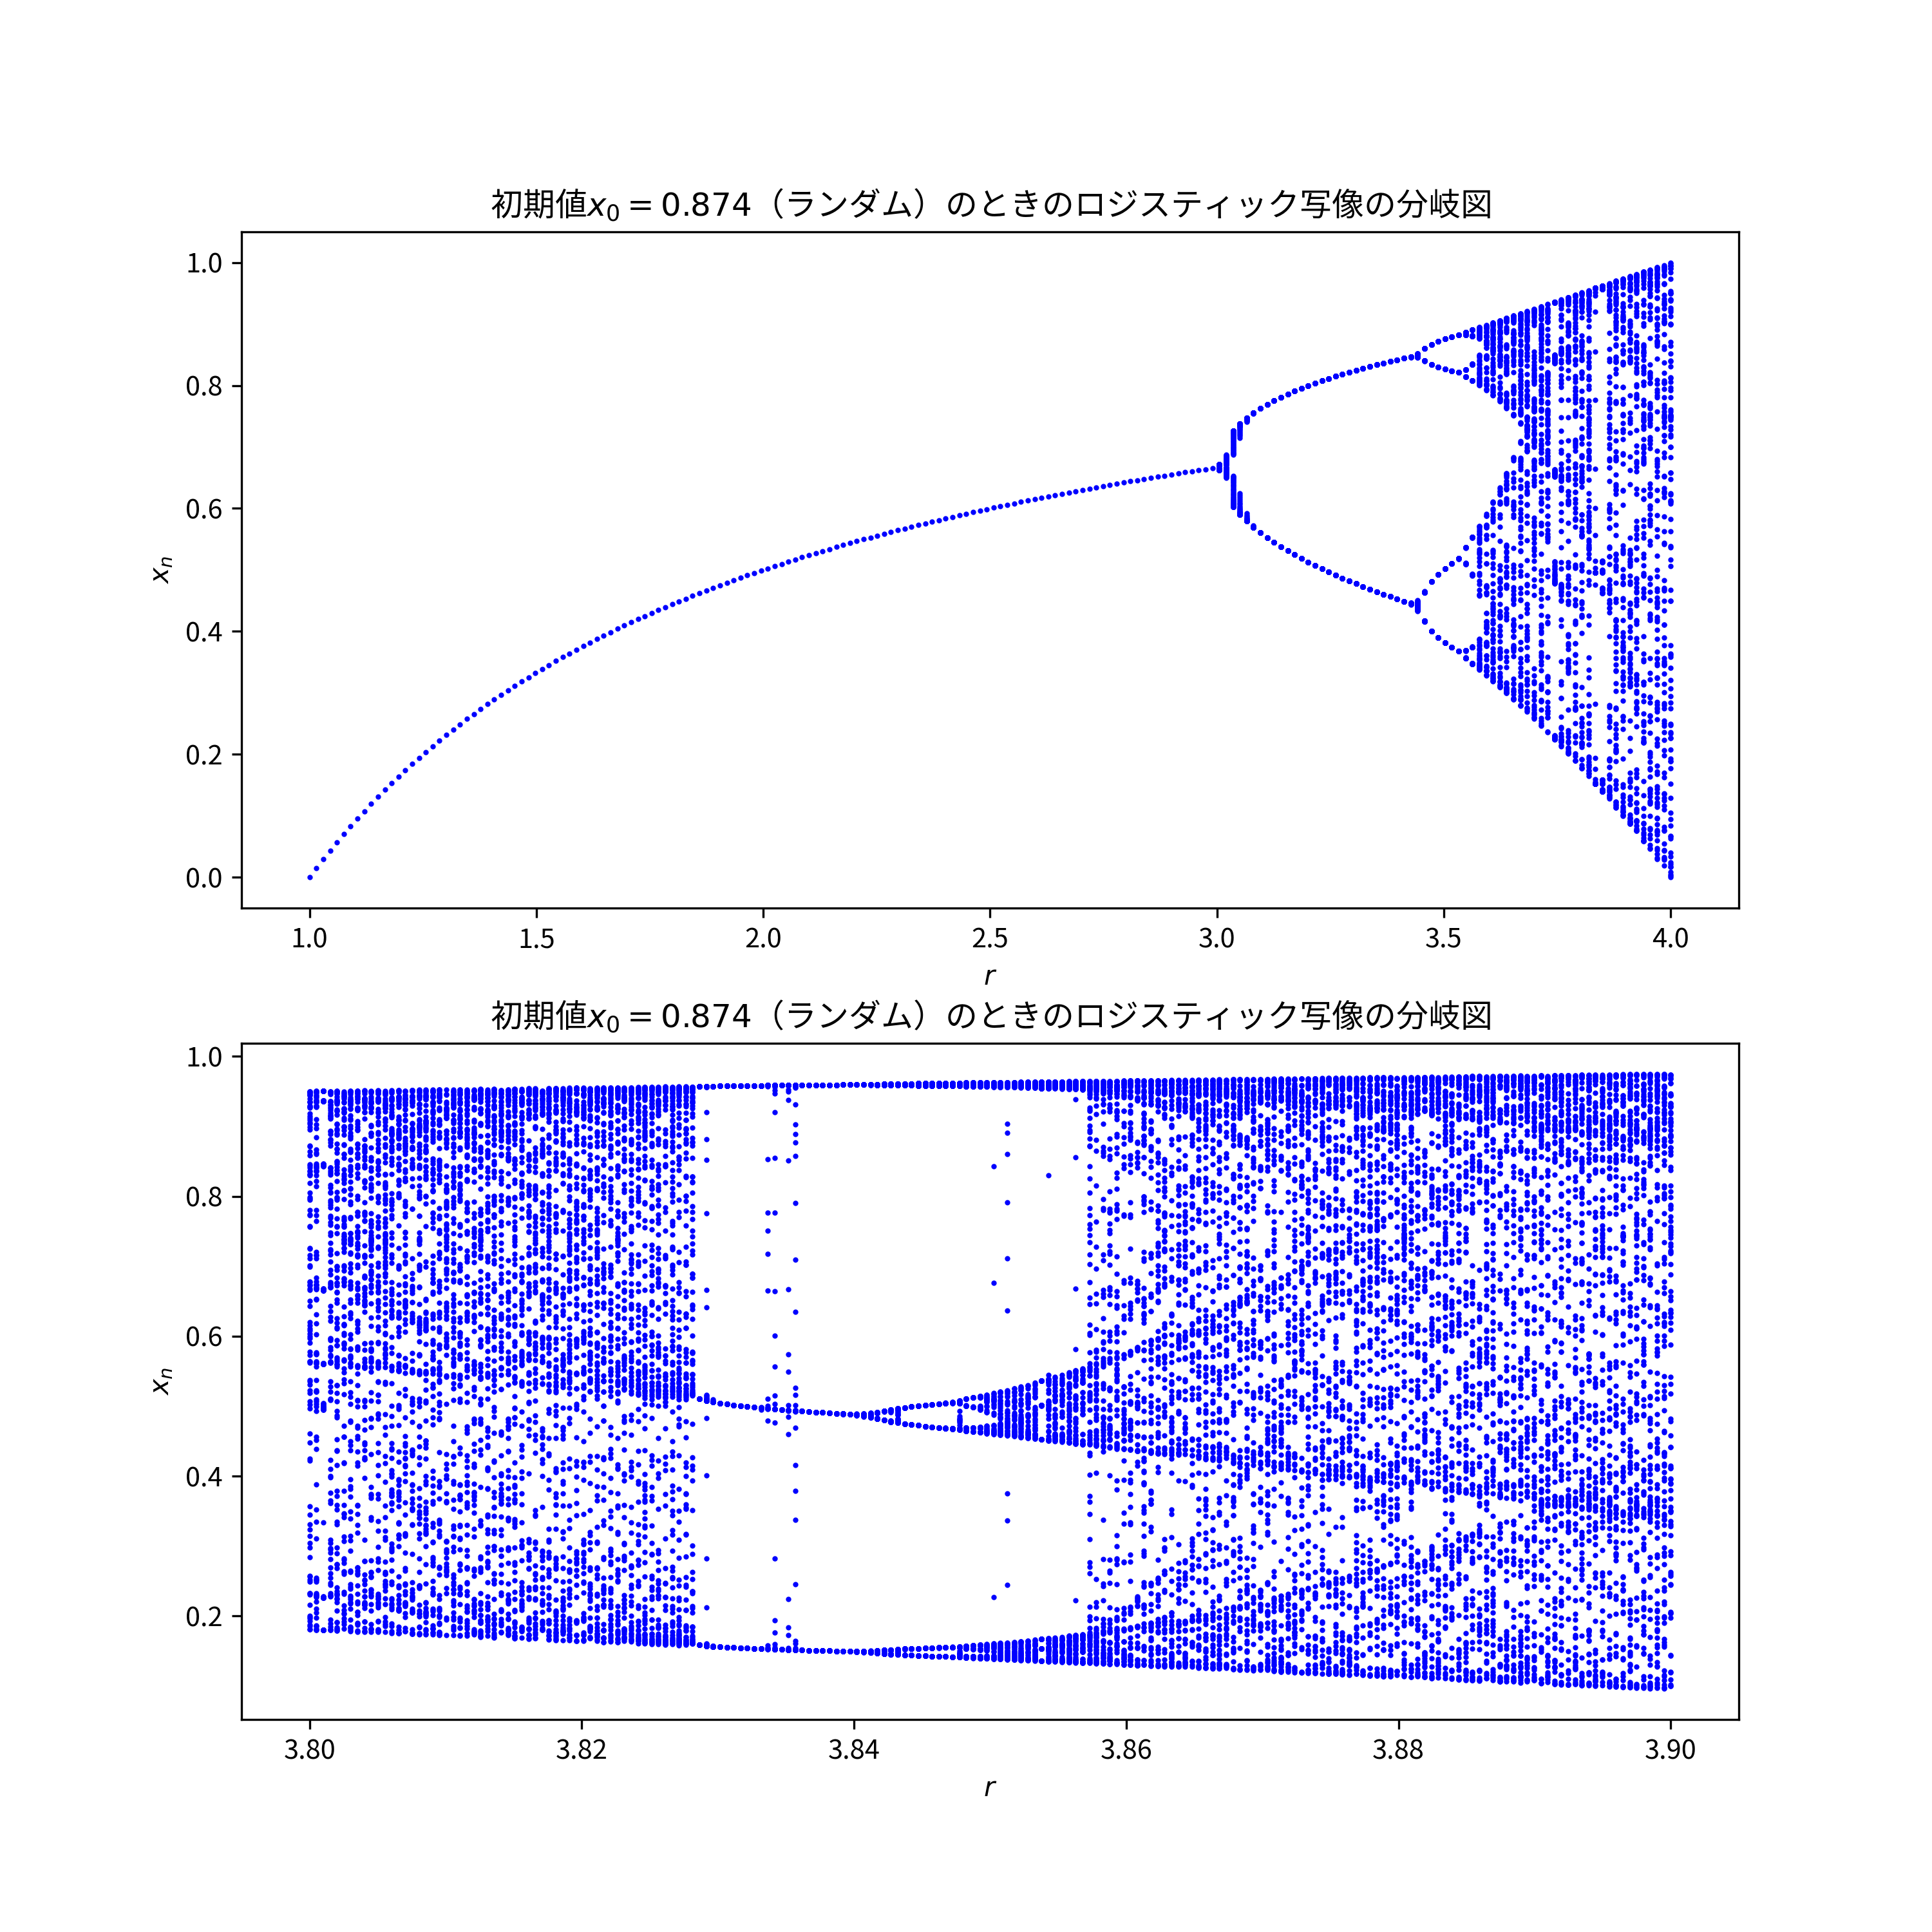
\includegraphics[keepaspectratio, scale=0.6]{images/Problem3/ctest4.png}
\end{figure}
\\
結果:\\
この画像から読み取れた。\\\\
考察:\\
これらの結果から考察することができる。

\subsection{課題3}
課題1と課題2は、各 $r$ ごとに初期値 $x_0$ をランダムに与えているにもかかわらず、 $r$ が $1~3.5$ くらいまでは何度プログラムを実行しても同じようなグラフを描くことができる。一方、 $r$ が $3.5$ よりも大きくなっていくと、プログラムを実行するたびにグラフを一見するだけではわからないような違いが生じる。この理由を前回の課題と初期値鋭敏性という言葉を用いて説明せよ。